% Trying to break the document up a bit.  This command simply inserts the contents of the file at this point.  It contains the document license, preamble, and title page: things that aren't likely to change more than once.  This can be used to separate discrete parts of a document into files that are easier to edit at one time.
%%%%%%%%%%%%%%%%%%%%%%%%%%%%%%%%%%%%%%%%%%%%%%%%%%%%%%%%%%%%%%%%%%%%%%
% This layout was adapted from one found at latextemplates.com which
% was adapted from another.
%
% License: CC BY-NC-SA 3.0
% (http://creativecommons.org/licenses/by-nc-sa/3.0/)
%
% Original header:
%
% This is a LaTeX version of the sample laboratory report from
% Virginia Tech's copyrighted 08-09 CHEM 1045/1046 lab manual.
% Reproduction of this one appendix section for academic purposes
% should fall under fair use.
%
%%%%%%%%%%%%%%%%%%%%%%%%%%%%%%%%%%%%%%%%%%%%%%%%%%%%%%%%%%%%%%%%%%%%%%

\documentclass{article}

\usepackage{graphicx}
% \usepackage[acronym]{glossaries} % Lets us use acronyms
\usepackage{multicol}
\usepackage{amsmath}
\usepackage{siunitx} % SI units in math mode
\usepackage{subcaption}

\author{}
\title{ELEC-313 \\ Lab 5: CMOS Circuits\\ }
\date{\today}

% \loadglsentries{acronyms} % Actually loads 'acronyms.tex'
% \makeglossaries

\begin{document}

\maketitle

\begin{center}
  \begin{tabular}{lr}
    Date Performed: & October 16, 2013 \\
    Partners:       & Charles Pittman    \\
    & Stephen Wilson     \\
  \end{tabular}
\end{center}

\newpage

\tableofcontents
\listoffigures
\listoftables
\newpage

% Number the enumerate environment (unordered lists) by letter:
\renewcommand{\labelenumi}{\alph{enumi}.}

\section{Objective}
\label{sec:objective}

\section{Equipment}
\label{sec:equipment}

\begin{tabular}{ll}
  \centering
  Transistor: 2N7000               & Power supply: HP E3631A            \\
  Function generator: HP 33120 & Multimeter: HP 34401A              \\
  Oscilloscope: Agilent 54622D & Capacitors: \SI{0.1}{\micro\farad} \\
  \multicolumn{2}{l}{Resistors: \SI{100}{\ohm}, \SI{300}{\ohm}, \SI{470}{\ohm}, \SI{1}{\kilo\ohm} (x2) \SI{33}{\kilo\ohm}, \SI{100}{\kilo\ohm} (x2)} \\
\end{tabular}

\section{Schematics}
\label{sec:schematics}

% \begin{figure}[hbtp]
%   \centering
%   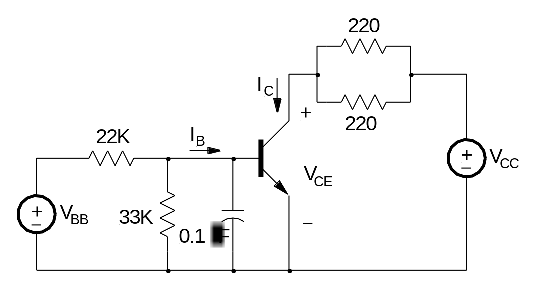
\includegraphics[width=0.6\textwidth]{circuit}
%   \caption{\label{fig:circuit} Circuit used in this lab.}
% \end{figure}

% \begin{figure}[hbtp]
%   \centering
%   \begin{subfigure}[b]{0.5\textwidth}
%     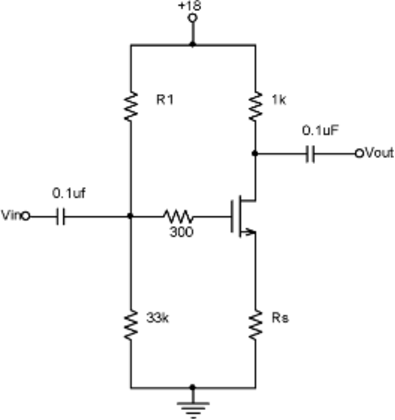
\includegraphics[width=\textwidth]{common-source}
%     \caption{\label{schem:common-source} Common-source amplifier}
%   \end{subfigure}%
%   ~
%   \begin{subfigure}[b]{0.5\textwidth}
%     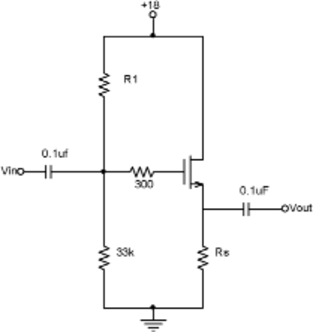
\includegraphics[width=\textwidth]{source-follower}
%     \caption{\label{schem:source-follower} Source-follower amplifier}
%   \end{subfigure}
%   \caption{\label{fig:schematics} Circuits used in this lab. $R_1=\SI{100}{\kilo\ohm}$,  $R_s=\SI{470}{\ohm}$}
% \end{figure}

\section{Procedure}
\label{sec:procedure}

% The following procedures were identified to observe the basic operation of MOSFET amplifier circuits.

% \subsection{Common-Source Amplifier}

% \begin{enumerate}
% \item Build the circuit shown in Figure~\ref{schem:common-source}.  Use the closest resistor values available for R1 and Rs.
% \item Measure and record the drain current and DC voltages at all terminals of the MOSFET.
% \item Set the function generator for a \SI{200}{V_{pp}}, \SI{20}{kHz} sine wave with \SI{0}{VDC} offset.  Connect it to $V_{in}$.
% \item Connect a \SI{100}{\kilo\ohm} load resistor from $V_{out}$ to ground.  This will be considered a no-load scenario.
% \item Connect channel 1 of the oscilloscope to $V_{in}$ and channel 2 to $V_{out}$.  Set the scope to trigger off of channel 1.
% \item Adjust the function generator to an amplitude of \SI{200}{V_{pp}} as measured on channel 1 of the oscilloscope.
% \item Measure the peak-to-peak output voltage on channel 2 of the oscilloscope.
% \item Repeat step 6 for input voltages of 300, 400, 500, 600, 700, 800, 900, and \SI{1000}{mV_{pp}}.
% \item Replace the \SI{100}{\kilo\ohm} from $V_{out}$ to ground with a \SI{1}{\kilo\ohm} load resistor.
% \item Reset the function generator to an amplitude of \SI{200}{V_{pp}} as measured on channel 1 of the oscilloscope.
% \item Measure the peak-to-peak output voltage on channel 2 of the oscilloscope.
% \end{enumerate}

% \subsection{Source-Follower Amplifier}

% \begin{enumerate}
% \item Construct the circuit shown in Figure~\ref{schem:source-follower} by removing the \SI{1}{\kilo\ohm} drain resistor and moving the output capacitor to the source of the MOSFET.
% \item Measure and record the drain current and DC voltages at all terminals of the MOSFET.
% \item Connect a \SI{100}{\kilo\ohm} load resistor from $V_{out}$ to ground. This will be considered a no-load scenario.
% \item Adjust the function generator to an amplitude of \SI{200}{V_{pp}} as measured on channel 1 of the oscilloscope.
% \item Measure the peak-to-peak output voltage on channel 2 of the oscilloscope.
% \item Repeat step 4 for input voltages of 300, 400, 500, 600, 700, 800, 900, and \SI{1000}{mV_{pp}}.
% \item Reset the function generator to an amplitude of \SI{200}{V_{pp}} as measured on channel 1 of the oscilloscope.
% \item Replace the \SI{100}{\kilo\ohm} resistor from $V_{out}$ to ground with a \SI{1}{\kilo\ohm} resistor and measure the peak-to-peak output voltage on channel 2 of the oscilloscope.
% \item Replace the \SI{1}{\kilo\ohm} load resistor with a \SI{100}{ohm} load resistor and measure the peak-to-peak output voltage on channel 2 of the oscilloscope.
% \end{enumerate}

\section{Results}

%\subsection{Common-Source Amplifier}

% \begin{table}[hbtp]
%   \centering
%   \begin{tabular}{r|cccc}
%                            & $V_{G}$ (\si{V}) & $V_{D}$ (\si{V}) & $V_{S}$ (\si{V}) & $I_D$ (\si{mA}) \\
%     \hline
%     \textbf{Measured}      & 4.391            & 13.498           & 2.11             & 4.52            \\
%     \textbf{Theoretical}   & 4.466            & 14.000           & 2.4214           & 4.00            \\
%     \textbf{\% Difference} & 1.712\%          & 3.719\%          & 14.800\%         & 11.500\%        \\
%   \end{tabular}
%   \caption{\label{tab:tran_common} Transistor characteristics}
% \end{table}

% \begin{table}[hbtp]
%   \centering
%   \begin{tabular}{ccc}
%     $V_{in}$ (\si{mV}) & $V_{out}$ (\si{V}) & $A_V$ \\
%     \hline
%     200                & 0.382              & 1.91  \\
%     300                & 0.566              & 1.89  \\
%     400                & 0.760              & 1.90  \\
%     500                & 0.939              & 1.88  \\
%     600                & 1.140              & 1.90  \\
%     700                & 1.340              & 1.91  \\
%     800                & 1.530              & 1.91  \\
%     900                & 1.721              & 1.91  \\
%     1000               & 1.90               & 1.90  \\
%   \end{tabular}
%   \caption{\label{tab:common-source} Common-source amplifier}
% \end{table}

%\subsection{Source-Follower Amplifier}

% \begin{table}[hbtp]
%   \centering
%   \begin{tabular}{cccc}
%     $V_G$ & $V_D$ & $V_S$ & $I_D$ \\
%     \hline
%     \SI{4.391}{V} & \SI{18.003}{V} & \SI{2.12}{V} & \SI{4.579}{mA} \\
%   \end{tabular}
%   \caption{\label{tab:tran_follower} Transistor characteristics}
% \end{table}

% \begin{table}[hbtp]
%   \centering
%   \begin{tabular}{ccc}
%     $V_{in}$ (\si{mV}) & $V_{out}$ (\si{mV}) & $A_V$ \\
%     \hline
%     200                & 182                 & 0.910 \\
%     300                & 268                 & 0.893 \\
%     400                & 360                 & 0.900 \\
%     500                & 451                 & 0.902 \\
%     600                & 541                 & 0.902 \\
%     700                & 634                 & 0.906 \\
%     800                & 725                 & 0.906 \\
%     900                & 813                 & 0.903 \\
%     1000               & 906                 & 0.906 \\
%   \end{tabular}
%   \caption{\label{tab:source-follower} Source-follower amplifier}
%\end{table}

\begin{figure}[hbtp]
  \centering
  \resizebox{1.0\textwidth}{!}{% GNUPLOT: LaTeX picture with Postscript
\begingroup
  \makeatletter
  \providecommand\color[2][]{%
    \GenericError{(gnuplot) \space\space\space\@spaces}{%
      Package color not loaded in conjunction with
      terminal option `colourtext'%
    }{See the gnuplot documentation for explanation.%
    }{Either use 'blacktext' in gnuplot or load the package
      color.sty in LaTeX.}%
    \renewcommand\color[2][]{}%
  }%
  \providecommand\includegraphics[2][]{%
    \GenericError{(gnuplot) \space\space\space\@spaces}{%
      Package graphicx or graphics not loaded%
    }{See the gnuplot documentation for explanation.%
    }{The gnuplot epslatex terminal needs graphicx.sty or graphics.sty.}%
    \renewcommand\includegraphics[2][]{}%
  }%
  \providecommand\rotatebox[2]{#2}%
  \@ifundefined{ifGPcolor}{%
    \newif\ifGPcolor
    \GPcolortrue
  }{}%
  \@ifundefined{ifGPblacktext}{%
    \newif\ifGPblacktext
    \GPblacktextfalse
  }{}%
  % define a \g@addto@macro without @ in the name:
  \let\gplgaddtomacro\g@addto@macro
  % define empty templates for all commands taking text:
  \gdef\gplbacktext{}%
  \gdef\gplfronttext{}%
  \makeatother
  \ifGPblacktext
    % no textcolor at all
    \def\colorrgb#1{}%
    \def\colorgray#1{}%
  \else
    % gray or color?
    \ifGPcolor
      \def\colorrgb#1{\color[rgb]{#1}}%
      \def\colorgray#1{\color[gray]{#1}}%
      \expandafter\def\csname LTw\endcsname{\color{white}}%
      \expandafter\def\csname LTb\endcsname{\color{black}}%
      \expandafter\def\csname LTa\endcsname{\color{black}}%
      \expandafter\def\csname LT0\endcsname{\color[rgb]{1,0,0}}%
      \expandafter\def\csname LT1\endcsname{\color[rgb]{0,1,0}}%
      \expandafter\def\csname LT2\endcsname{\color[rgb]{0,0,1}}%
      \expandafter\def\csname LT3\endcsname{\color[rgb]{1,0,1}}%
      \expandafter\def\csname LT4\endcsname{\color[rgb]{0,1,1}}%
      \expandafter\def\csname LT5\endcsname{\color[rgb]{1,1,0}}%
      \expandafter\def\csname LT6\endcsname{\color[rgb]{0,0,0}}%
      \expandafter\def\csname LT7\endcsname{\color[rgb]{1,0.3,0}}%
      \expandafter\def\csname LT8\endcsname{\color[rgb]{0.5,0.5,0.5}}%
    \else
      % gray
      \def\colorrgb#1{\color{black}}%
      \def\colorgray#1{\color[gray]{#1}}%
      \expandafter\def\csname LTw\endcsname{\color{white}}%
      \expandafter\def\csname LTb\endcsname{\color{black}}%
      \expandafter\def\csname LTa\endcsname{\color{black}}%
      \expandafter\def\csname LT0\endcsname{\color{black}}%
      \expandafter\def\csname LT1\endcsname{\color{black}}%
      \expandafter\def\csname LT2\endcsname{\color{black}}%
      \expandafter\def\csname LT3\endcsname{\color{black}}%
      \expandafter\def\csname LT4\endcsname{\color{black}}%
      \expandafter\def\csname LT5\endcsname{\color{black}}%
      \expandafter\def\csname LT6\endcsname{\color{black}}%
      \expandafter\def\csname LT7\endcsname{\color{black}}%
      \expandafter\def\csname LT8\endcsname{\color{black}}%
    \fi
  \fi
  \setlength{\unitlength}{0.0500bp}%
  \begin{picture}(7200.00,5040.00)%
    \gplgaddtomacro\gplbacktext{%
      \csname LTb\endcsname%
      \put(726,440){\makebox(0,0)[r]{\strut{}0mA}}%
      \csname LTb\endcsname%
      \put(726,1307){\makebox(0,0)[r]{\strut{}5mA}}%
      \csname LTb\endcsname%
      \put(726,2174){\makebox(0,0)[r]{\strut{}10mA}}%
      \csname LTb\endcsname%
      \put(726,3041){\makebox(0,0)[r]{\strut{}15mA}}%
      \csname LTb\endcsname%
      \put(726,3908){\makebox(0,0)[r]{\strut{}20mA}}%
      \csname LTb\endcsname%
      \put(726,4775){\makebox(0,0)[r]{\strut{}25mA}}%
      \csname LTb\endcsname%
      \put(858,220){\makebox(0,0){\strut{}0 V}}%
      \csname LTb\endcsname%
      \put(1453,220){\makebox(0,0){\strut{}2 V}}%
      \csname LTb\endcsname%
      \put(2047,220){\makebox(0,0){\strut{}4 V}}%
      \csname LTb\endcsname%
      \put(2642,220){\makebox(0,0){\strut{}6 V}}%
      \csname LTb\endcsname%
      \put(3236,220){\makebox(0,0){\strut{}8 V}}%
      \csname LTb\endcsname%
      \put(3831,220){\makebox(0,0){\strut{}10 V}}%
      \csname LTb\endcsname%
      \put(4425,220){\makebox(0,0){\strut{}12 V}}%
      \csname LTb\endcsname%
      \put(5020,220){\makebox(0,0){\strut{}14 V}}%
      \csname LTb\endcsname%
      \put(5614,220){\makebox(0,0){\strut{}16 V}}%
      \csname LTb\endcsname%
      \put(6209,220){\makebox(0,0){\strut{}18 V}}%
      \csname LTb\endcsname%
      \put(6803,220){\makebox(0,0){\strut{}20 V}}%
    }%
    \gplgaddtomacro\gplfronttext{%
      \csname LTb\endcsname%
      \put(5816,4602){\makebox(0,0)[r]{\strut{}$I_B = $SI{20}{microampere}}}%
      \csname LTb\endcsname%
      \put(5816,4382){\makebox(0,0)[r]{\strut{}$I_B = $SI{50}{microampere}}}%
      \csname LTb\endcsname%
      \put(5816,4162){\makebox(0,0)[r]{\strut{}$I_B = $SI{80}{microampere}}}%
      \csname LTb\endcsname%
      \put(5816,3942){\makebox(0,0)[r]{\strut{}$I_B = $SI{100}{microampere}}}%
    }%
    \gplbacktext
    \put(0,0){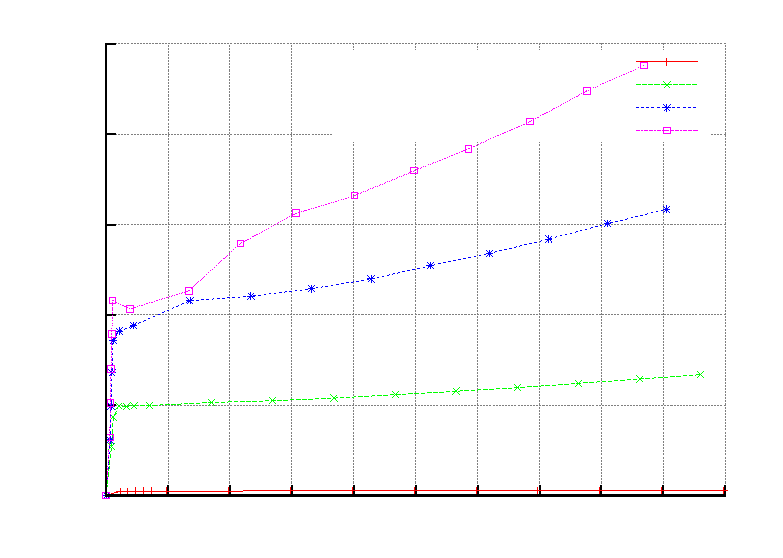
\includegraphics{graph}}%
    \gplfronttext
  \end{picture}%
\endgroup
}
  \caption{\label{fig:graph} $V_{CE}$ vs. $I_C$}
\end{figure}

\section{Conclusion}
\label{sec:conclusion}

\section{Equations}
\label{sec:equations}

% LaTeX sees blank lines as a start of another paragraph.  To avoid
% unnecessary vertical spaces between equations, and still visually
% separate in source, put a comment between them.
%
\begin{equation}
  \label{eq:amp}
  V_{o,L} = V_{o,NL} \frac{R_L}{R_o + R_L}
\end{equation}
%
\begin{equation}
  \label{eq:V_G}
  V_G = \frac{V_{DD} \cdot \SI{33}{\kilo\ohm}}{\SI{100}{\kilo\ohm} + \SI{33}{\kilo\ohm}}
\end{equation}
%
\begin{equation}
  \label{eq:V_S}
  V_S = V_G \cdot \sqrt{\frac{I_D}{K_N}} - V_{TN}
\end{equation}
%
\begin{equation}
  \label{eq:V_D}
  V_D = V_{DD} - I_D \cdot \SI{1}{\kilo\ohm}
\end{equation}
%
\begin{equation}
  \label{eq:I_D}
  I_D = \frac{V_S}{R_S}
\end{equation}
%
\begin{equation}
  \label{eq:A_V}
  A_V = \frac{V_{out}}{V_{in}} = \frac{-g_m \cdot R_D}{1 + g_m \cdot R_S}
\end{equation}
%
\begin{equation}
  \label{eqn:percent_diff}
  \%_{diff} = \frac{|measured - theoretical|}{theoretical} \times 100\%
\end{equation}

\end{document}
